\chapter{Opis projektnog zadatka}
		
		\textbf{\textit{dio 1. revizije}}\\
		
		\textit{Na osnovi projektnog zadatka detaljno opisati korisničke zahtjeve. Što jasnije opisati cilj projektnog zadatka, razraditi problematiku zadatka, dodati nove aspekte problema i potencijalnih rješenja. Očekuje se minimalno 3, a poželjno 4-5 stranica opisa.	Teme koje treba dodatno razraditi u ovom poglavlju su:}
		\begin{packed_item}
			\item \textit{potencijalna korist ovog projekta}
			\item \textit{postojeća slična rješenja (istražiti i ukratko opisati razlike u odnosu na zadani zadatak). Dodajte slike koja predočavaju slična rješenja.}
			\item \textit{skup korisnika koji bi mogao biti zainteresiran za ostvareno rješenje.}
			\item \textit{mogućnost prilagodbe rješenja }
			\item \textit{opseg projektnog zadatka}
			\item \textit{moguće nadogradnje projektnog zadatka}
		\end{packed_item}
		
		\textit{Za pomoć pogledati reference navedene u poglavlju „Popis literature“, a po potrebi konzultirati sadržaj na internetu koji nudi dobre smjernice u tom pogledu.}
		\eject
		
		 U ovo moderno doba i vrijeme, kada su tehnološka sredstva uvijek nadomak ruke, nekolicina entuzijasta se dosjetila kako doskočiti u pomoć svom gradu. Naime, štete po cestama i javnim provršinama se ne smanjuju, ali to je upravo cilj jednog ovakvog projekta. \\
		
		 Ono što ovaj projekt nastoji ponuditi jest upravo jedno pravo suvremeno i efikasno rješenje pristupačno svima a usmjereno samo prema jednoj stvari - prijavljivanje štete javnih površina u gradu. Cilj projekta je svim ljudima omogućiti jednostavni pristup aplikaciji preko koje će moći prijavljivati uočena oštećenja javnih površina i cesta u područjima gradova čime sveukupno kumulira poboljšanje života u društvu.\\
		
		 Ukratko, tijek zamišljenih događaja je idući: Korisnik uoči oštećenu gradsku imovinu ili cestu te istu želi prijaviti gradskom uredu nadležnom za taj tip štete. Korisnik učitava našu aplikacuju te šalje prijavu sa određenim popunjenim podacima. Gradski ured dobiva obavijest o prijavi te kad istu riješi korisnik koji ju je prijavio dobiva obavijest da je ona razriješena. \\
		
		 Pri učitavanju početne stranice aplikacije korisniku je vidljiva karta, opcija za registraciju (ili prijavu), te opcija za podnošenje prijave. Regsistririani kao i neregistrirani korisnici imaju mogućnost slanja prijave, ali razlika je u tome što neregistrirani korisnik dobiva jedinstveni broj pomoću kojeg prati status prijave, registrirani korisnik uvijek može samo ući u povijest svojih prijava i vidjeti status svake.
		
		 Neregistrirani korisnik se u svakom trenutku može regitrirati, te pri registraciji trebe navesti iduće podatke:
		
		\begin{packed_item}
		\item Ime
		\item Prezime
		\item Korisničko ime
		\item E-mail
		\item Lozinku\\
		\end{packed_item}
		
		 Registrirani korisnici se uvijek mogu prijaviti u sustav pomoću svog korisničkog imena i lozinke. Ako je korisnik prijavljen u sustav, ima mogućnost odjave ponuđenu u gornjem desnom kutu.
		\noindent Registrirani korisnici su podijeljeni na iduć uloge:
			\begin{packed_item}
			\item Klijent
			\item Administrator
			\item Gradski ured\\
			\end{packed_item}
			
			Klijent na karti ima označene sve aktivne prijave. Pri pregledu prijava, prijave može filtrirati po tematici (tipu) i lokaciji. Pri predaji prijave, korsinik mora unijeti iduće podatke:
			\begin{packed_item}
			\item Naziv
			\item Kratki opis
			\item Geografske koordinate
			\end{packed_item}
			
			Uz sve to, korisnik ocionalno može poslati i sliku viđenog pa sustav, u slučaju da nisu unesene koordinate, langituda i longituda se daju pročitati sa meta podataka fotografije. Web stranica koja  nudi sličnu uslugu, ali je bazirana na vandalizmu i isključivo grafitima u Londonu je: \\ \url{https://www.newham.gov.uk/publichealth-safety/graffiti-reporting-removal}, a izgled je na slici \ref{fig:promjene}.\\
			
			\begin{figure}[H]
			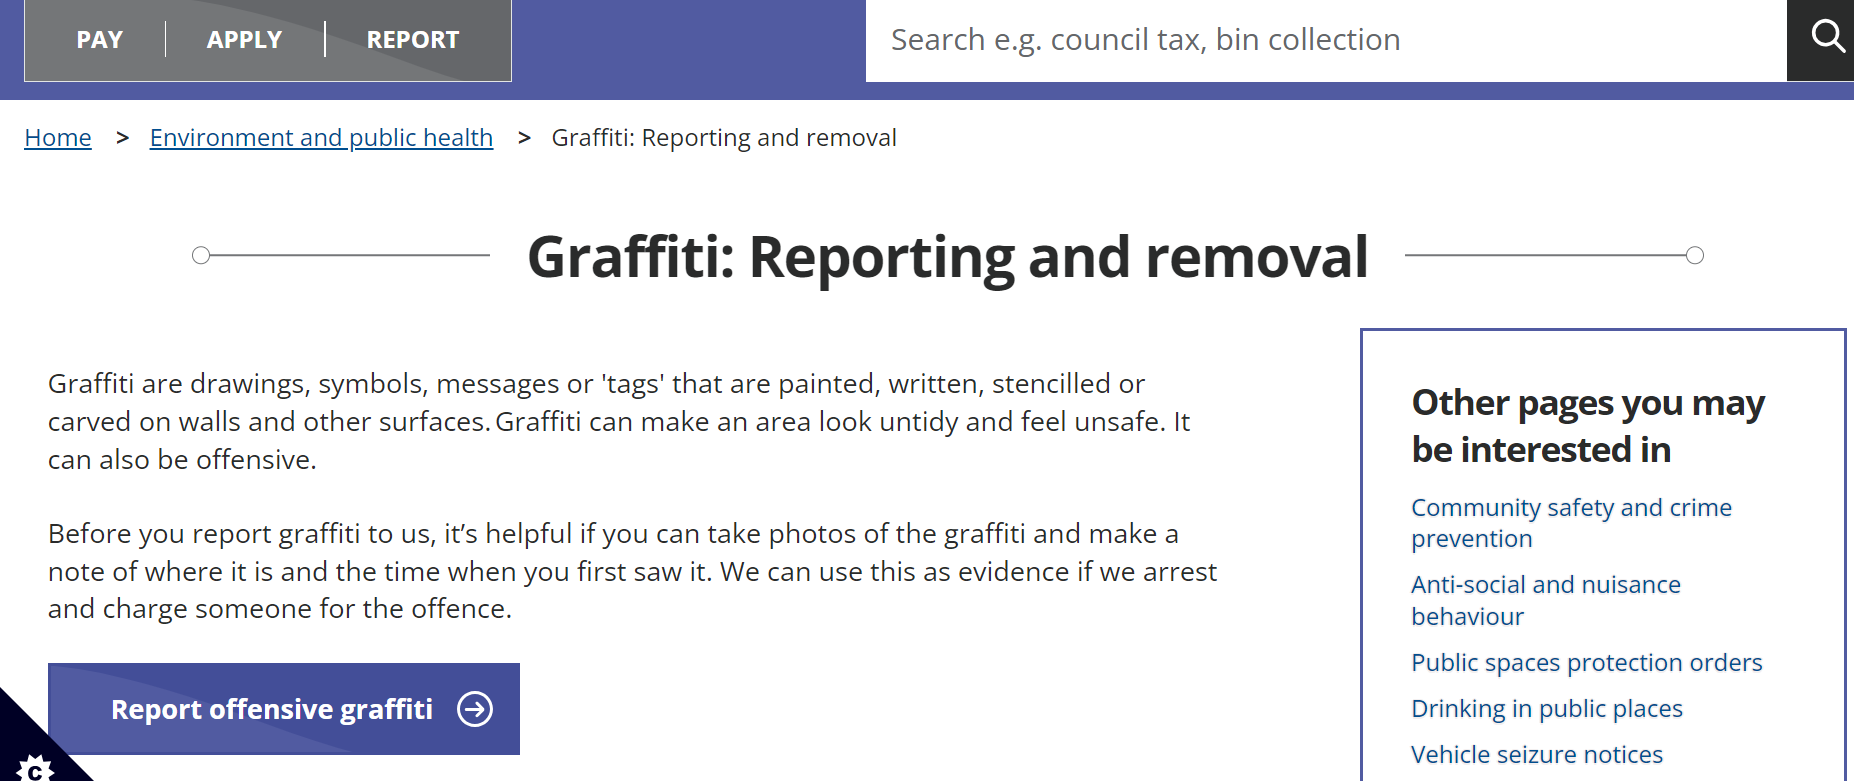
\includegraphics[scale=0.4]{slike/simular_page.PNG} %veličina slike u odnosu na originalnu datoteku i pozicija slike
			\centering
			\caption{Izgled navedene stranice}
			\label{fig:promjene}
		\end{figure}
		
		Administrator je uloga koja ima najveće ovlasti. On je tu da kontrolira sve vezano za stranicu pa tako ima mogućnost uređivanja podataka pojedinih prijava kojen smatra nevaljalima kao i njihovo brisanje iz baze podatka. Pored toga, može briasti profile regsitriranih korsinika za koje procjeni da krše pravila ponašanja na aplikaciji. 
		
		Uz navedene korisnike sustava, još postoje i gradski uredi koji primaju prijave na temelju tematike problema za koju su zaduženi. Tako će puknuće na cestama primati isključivo javni zavod za ceste, probleme sa zgradama će obrađivati ured za izgradnju i prostorno uređenje, probleme sa vodovom ured za vodovod...  Dodatno, svaki gradski ured uvijek ima mogućnost  promjene statusa prijave koji će prijaviteljima omogućiti da jasno vide ukoliko je prijava razriješena ili nije. Uz to, ured može povezati one prijave koje korisnici nisu povezali ukoliko shvati da se radi o istom problemu iste tematike.\\
		
		Sustav će sve prijave obrađivati u stvarnom vremenu pa će korisnici u bilo kojem trenutku iamti uvid da li je npr. neko puknuće na cesti razriješeno te da li se tom cestom promet uopće može odvijati. Sličnu mogućnost nudi stranica HAK-a na idućoj adresi : \url{https://www.hak.hr/info/stanje-na-cestama/#prohodnost-cesta} na slici ref{hak}.\\
		
			
			\begin{figure}[H]
			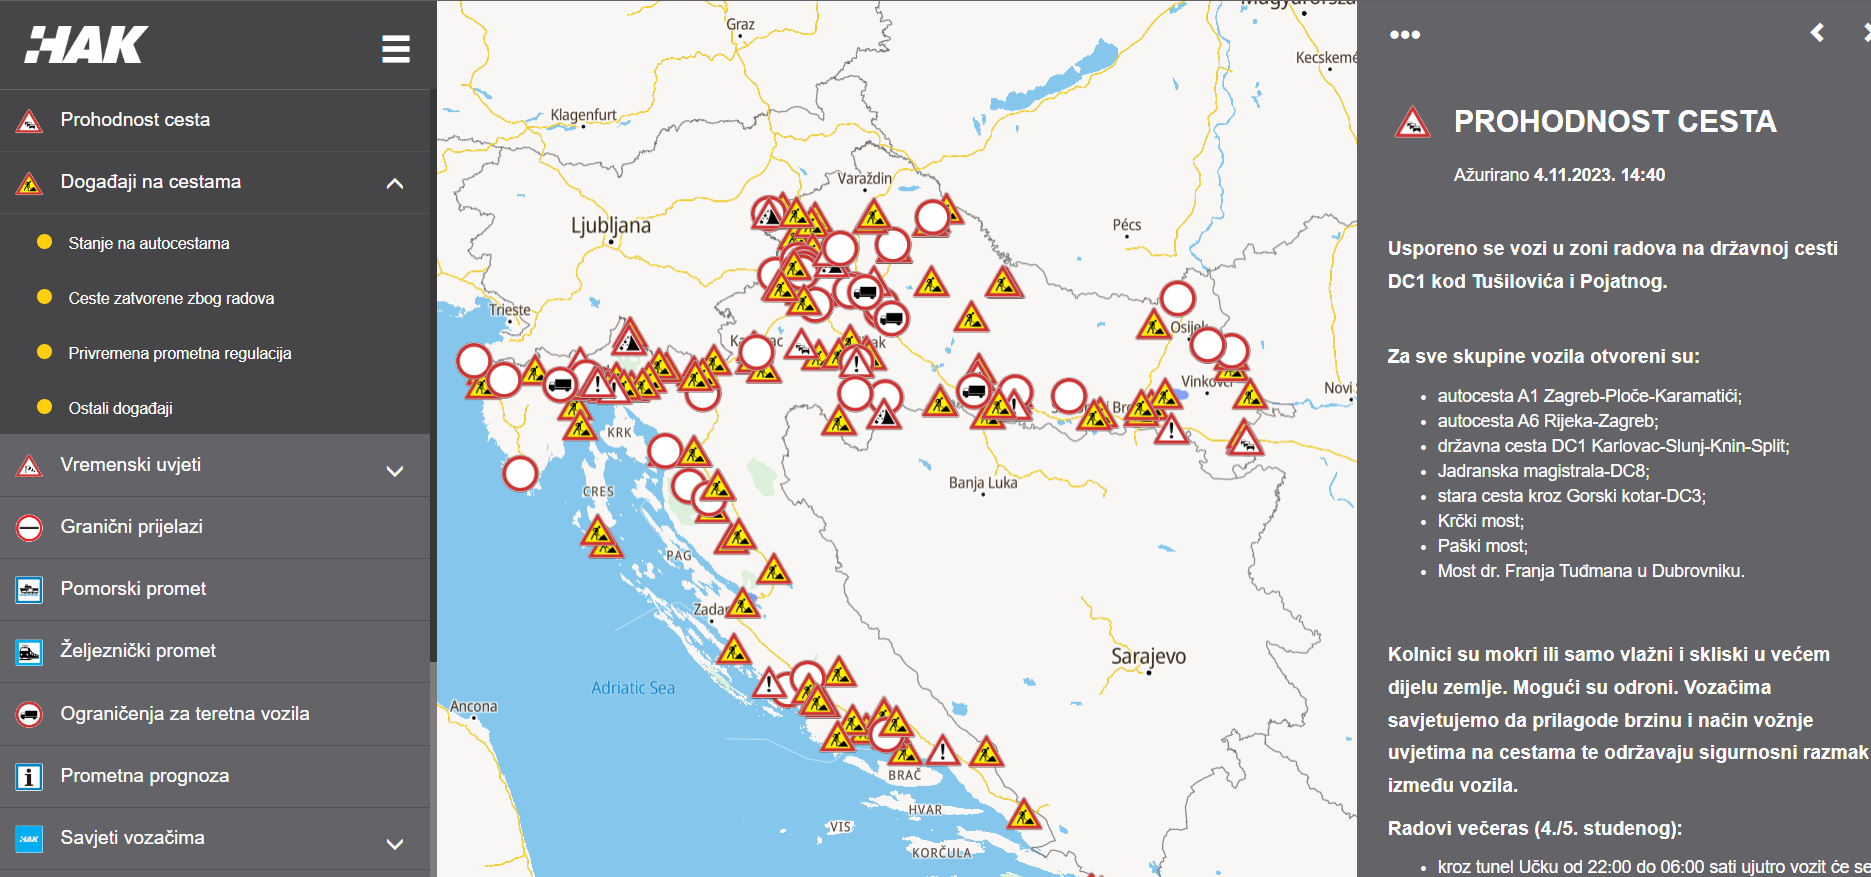
\includegraphics[scale=0.4]{slike/hak.PNG} %veličina slike u odnosu na originalnu datoteku i pozicija slike
			\centering
			\caption{HAK - stanje na cestama}
			\label{fig:hak}
		\end{figure}
		
		
		
		Ovakva aplikacije sama po sebi već ima klijentelu i predispozicije za uspješno korištenje i popularizaciju. Uz štete javnih površina i cesta moglo bi se dodati prijava za zastoj primjerice tramvaja na određenoj lokaciji (naravmo u gradovima gdje je tramvajski prijevoz omogućen) kako bi bilo vidljivo svim korisnicima aplikacije u stavrnom vremenu. Uz to moglo bi se podriučje aplikacije proširiti na prometne nesreće kako bi korisnici uz status da li je cesta zatvorena ili ne, mogli uz sliku procijeniti prohodnost iste. Neke vizualne stvari za krosinike koje se mogu još dodati bi bile gledanje tuđih profila, kao i dopisivanje porukama kako bi se doznale konkretnije informacije o prijavi od osobe koja je tu prijavu napravila. Kako je Hrvatska turistička zemlja, aplikaciji bi se još mogli dodati ostali osnovni jezici za inozemne korisnike. Kako bi se što više promoviralo prijavljivanje šteta, u aplikaciju bi se dala ugraditi neka online nagrađivanja; primjerice dostupnost povećanja levela i stjecanja points-a.
		
		
		
		
		
		\section{Primjeri u \LaTeX u}
		
		\textit{Ovo potpoglavlje izbrisati.}\\

		U nastavku se nalaze različiti primjeri kako koristiti osnovne funkcionalnosti \LaTeX a koje su potrebne za izradu dokumentacije. Za dodatnu pomoć obratiti se asistentu na projektu ili potražiti upute na sljedećim web sjedištima:
		\begin{itemize}
			\item Upute za izradu diplomskog rada u \LaTeX u - \url{https://www.fer.unizg.hr/_download/repository/LaTeX-upute.pdf}
			\item \LaTeX\ projekt - \url{https://www.latex-project.org/help/}
			\item StackExchange za Tex - \url{https://tex.stackexchange.com/}\\
		
		\end{itemize} 	


		
		\noindent \underbar{podcrtani tekst}, \textbf{podebljani tekst}, 	\textit{nagnuti tekst}\\
		\noindent \normalsize primjer \large primjer \Large primjer \LARGE {primjer} \huge {primjer} \Huge primjer \normalsize
				
		\begin{packed_item}
			
			\item  primjer
			\item  primjer
			\item  primjer
			\item[] \begin{packed_enum}
				\item primjer
				\item[] \begin{packed_enum}
					\item[1.a] primjer
					\item[b] primjer
				\end{packed_enum}
				\item primjer
			\end{packed_enum}
			
		\end{packed_item}
		
		\noindent primjer url-a: \url{https://www.fer.unizg.hr/predmet/proinz/projekt}
		
		\noindent posebni znakovi: \# \$ \% \& \{ \} \_ 
		$|$ $<$ $>$ 
		\^{} 
		\~{} 
		$\backslash$ 
		
		
		\begin{longtblr}[
			label=none,
			entry=none
			]{
				width = \textwidth,
				colspec={|X[8,l]|X[8, l]|X[16, l]|}, 
				rowhead = 1,
			} %definicija širine tablice, širine stupaca, poravnanje i broja redaka naslova tablice
			\hline \SetCell[c=3]{c}{\textbf{naslov unutar tablice}}	 \\ \hline[3pt]
			\SetCell{LightGreen}IDKorisnik & INT	&  	Lorem ipsum dolor sit amet, consectetur adipiscing elit, sed do eiusmod  	\\ \hline
			korisnickoIme	& VARCHAR &   	\\ \hline 
			email & VARCHAR &   \\ \hline 
			ime & VARCHAR	&  		\\ \hline 
			\SetCell{LightBlue} primjer	& VARCHAR &   	\\ \hline 
		\end{longtblr}
		

		\begin{longtblr}[
				caption = {Naslov s referencom izvan tablice},
				entry = {Short Caption},
			]{
				width = \textwidth, 
				colspec = {|X[8,l]|X[8,l]|X[16,l]|}, 
				rowhead = 1,
			}
			\hline
			\SetCell{LightGreen}IDKorisnik & INT	&  	Lorem ipsum dolor sit amet, consectetur adipiscing elit, sed do eiusmod  	\\ \hline
			korisnickoIme	& VARCHAR &   	\\ \hline 
			email & VARCHAR &   \\ \hline 
			ime & VARCHAR	&  		\\ \hline 
			\SetCell{LightBlue} primjer	& VARCHAR &   	\\ \hline 
		\end{longtblr}
	


		
		
		%unos slike
		\begin{figure}[H]
			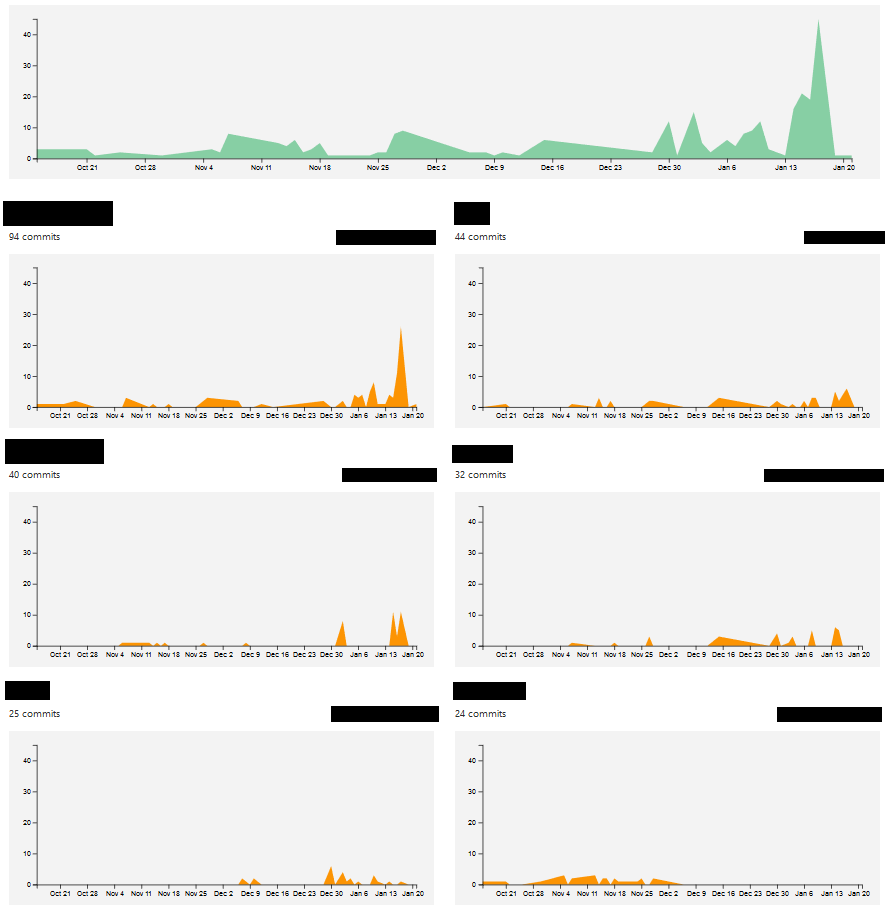
\includegraphics[scale=0.4]{slike/aktivnost.PNG} %veličina slike u odnosu na originalnu datoteku i pozicija slike
			\centering
			\caption{Primjer slike s potpisom}
			\label{fig:promjene1}
		\end{figure}
		
		\begin{figure}[H]
			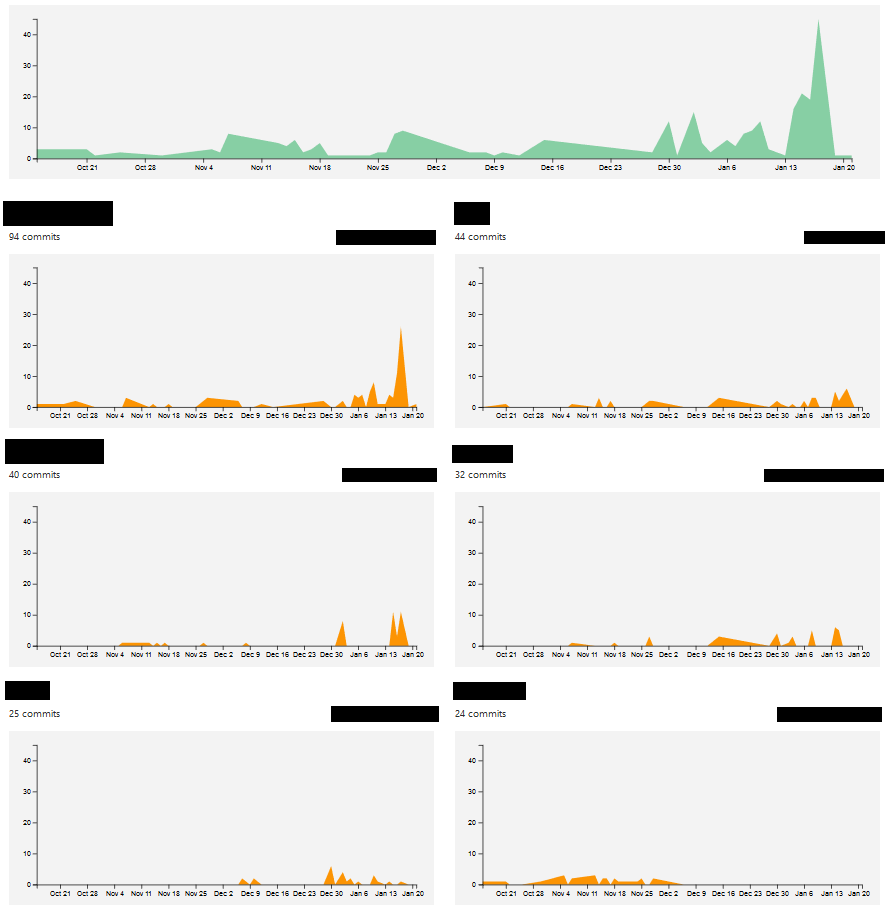
\includegraphics[width=\textwidth]{slike/aktivnost.PNG} %veličina u odnosu na širinu linije
			\caption{Primjer slike s potpisom 2}
			\label{fig:promjene2} %label mora biti drugaciji za svaku sliku
		\end{figure}
		
		Referenciranje slike \ref{fig:promjene2} u tekstu.
		
		\eject
		
	